\documentclass[11pt]{article}
\usepackage{../header}

\def\title{Differential Equations}

\begin{document}
\maketitle
\tableofcontents
\newpage

\section{RC circuits}

Consider a charged capacitor that is slowly discharging through this circuit:

\begin{figure}[H]
    \centering
        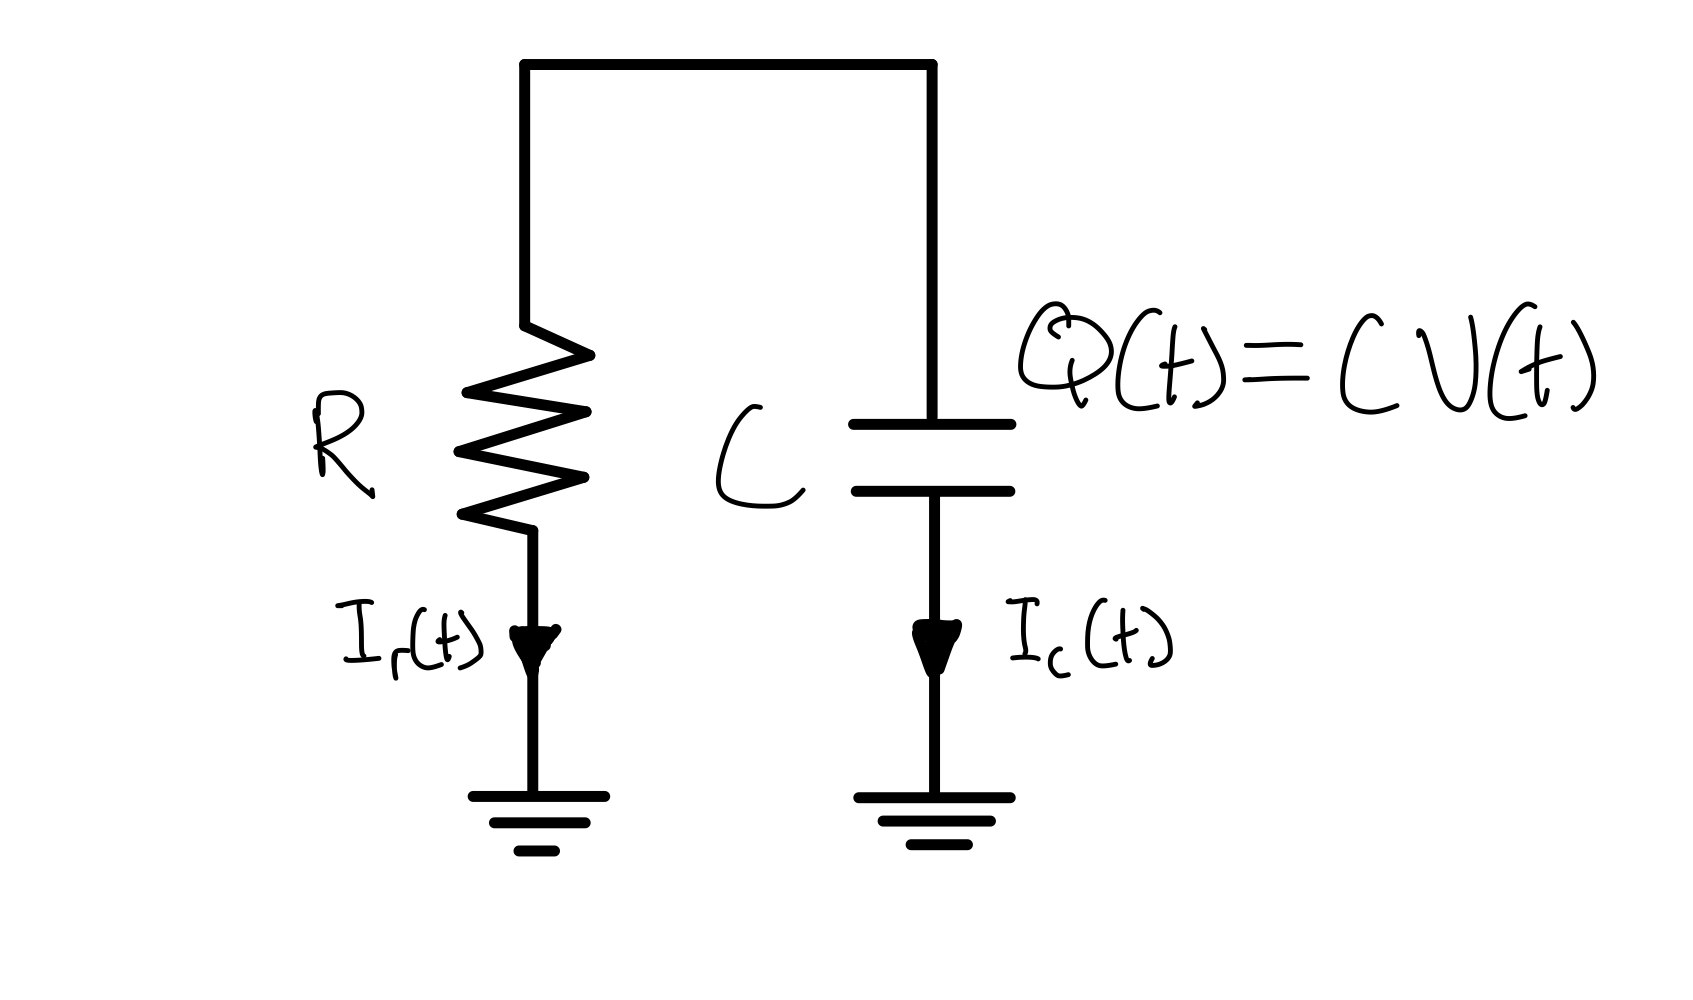
\includegraphics[scale=.12]{02-diffeq/simple-rc.jpeg}
    \caption{Simple RC circuit}
\end{figure}

Recall the circuit formulas from EECS 16A:

\begin{align}
    V&=IR\\
    Q&=CV
\end{align}

Since $V,I,Q$ change over time in this system, we represent them as the functions $V(t),I(t),Q(t)$ instead.

The charge $Q(t)$ of the capacitor gradually decreases via the resistor, proportional to the current at the resistor $I(t)=\frac{V(t)}{R}$. However, since $V(t)$, and thus $I(t)$, depends on $Q(t)$, the current decreases as the charge depletes, and the rate at which the capacitor discharges slows down too. 

Intuitively, the graph of $V(t)$ over time would have some initial slope, and then gradually flatten out as it approaches zero.

\begin{figure}[H]
    \centering
        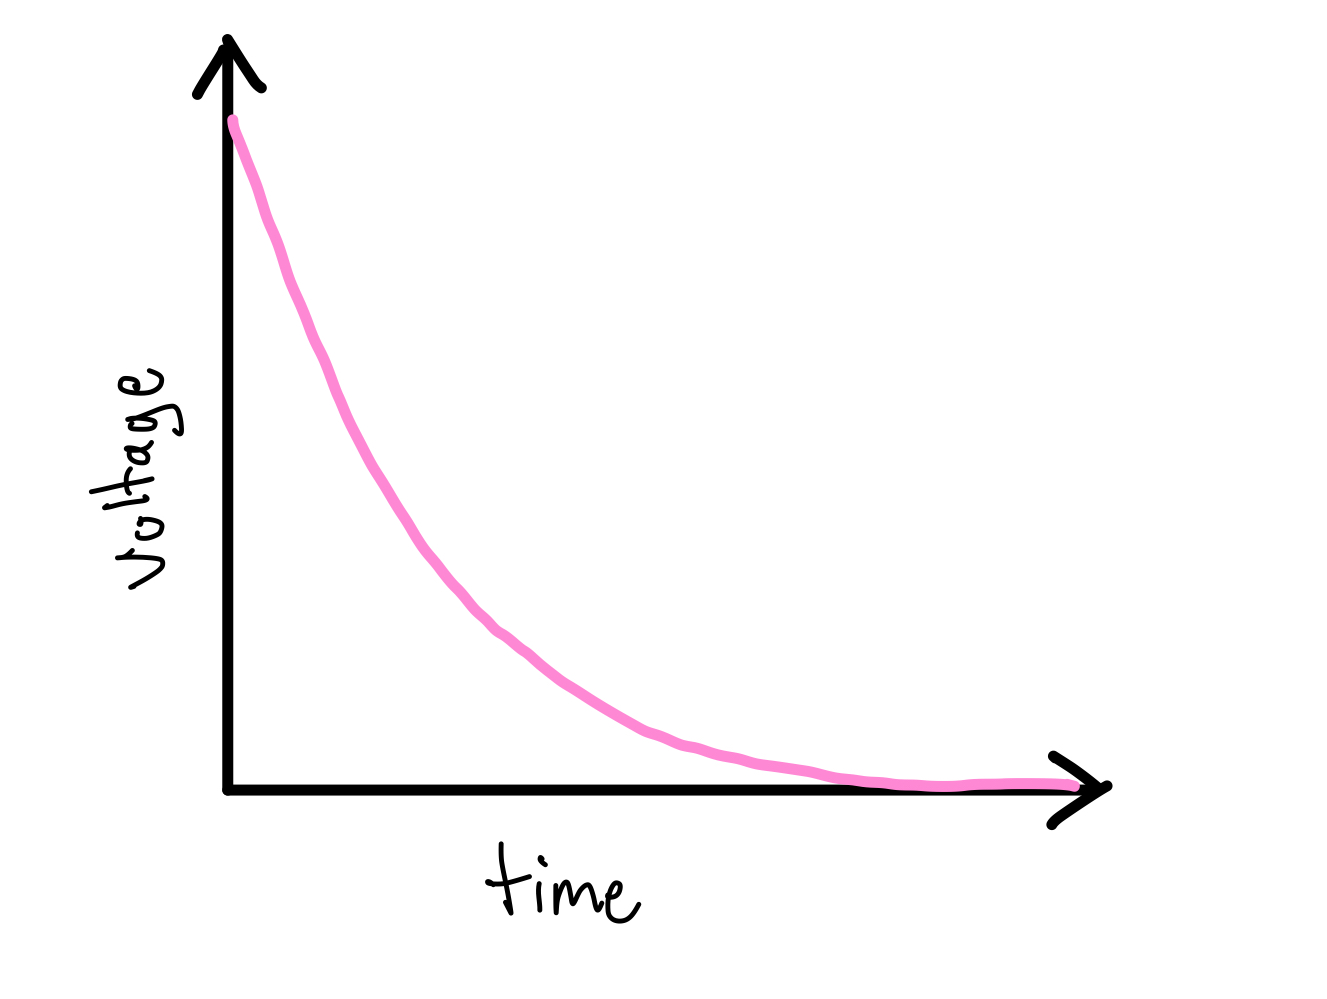
\includegraphics[scale=.15]{02-diffeq/discharge-estimate.jpeg}
    \caption{Voltage on capacitor discharging through resistor}
\end{figure}

\subsection{Mathematical approach}
Now, let's do some math to figure out exactly how the voltage changes.

The two currents are facing opposite directions, so we get \[I_c(t)=-I_r(t)\]

Recall from 16A that current is defined as charge over time \[I_c(t)=\frac d{dt}Q(t)=C\frac d{dt}V(t)\]

Finally, the last equation we need is \[I_r(t)=\frac{V(t)}{R}\]

Substituting some variables in these equations yields us an equation that relates $V(t)$ to its derivative: \[\frac d{dt}V(t)=-\frac{V(t)}{RC}\]

An equation in this form, relating the derivative of a function to something, is called a differential equation. We'll learn how to solve them in the next section.

\subsection{Revisiting inverters}

Let's revisit oscillators in the Transistors note, where the inverters were connected in a sequence. Suppose the first inverter was outputting 1 (high) for a long time, and then switched to 0 (low). 

The capacitors have been charged with a voltage of $V_{DD}$ for a long time and have just been switched to instead be connected to a resistor that leads to ground.

\begin{figure}[H]
    \centering
        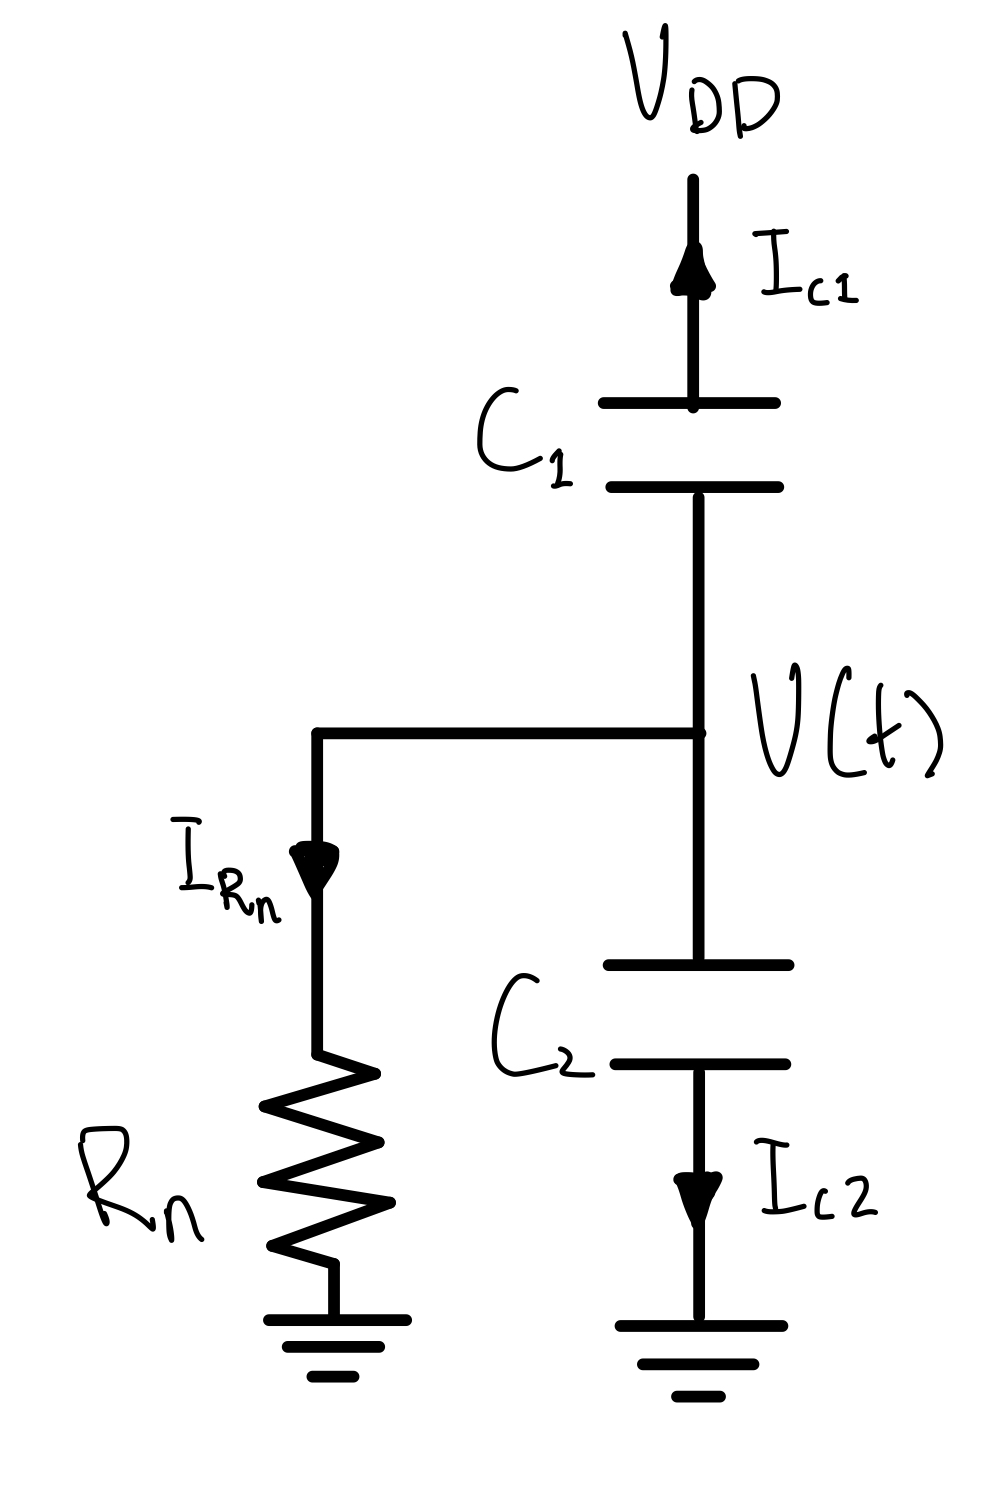
\includegraphics[scale=.12]{02-diffeq/inverter.jpeg}
    \caption{The low output of one inverter connected to the input of another inverter}
\end{figure}

Same as the previous circuit, we know how the current relates to the voltage across the resistor: \[I_{R_n}=\frac{V(t)}{R_n}\]

Since the voltage across $C_1$ is $V(t)-V_{DD}$ and the voltage across $C_2$ is $V(t)$, we get that
\begin{align*}
    I_{c1}&=C_1\frac d{dt}(V(t)-V_{DD})\\
    I_{c2}&=C_2\frac d{dt}V(t)
\end{align*}

Finally, from KCL, we know the sum of all the currents is zero, and from there we can solve for $V(t)$
\begin{align*}
    I_{c1}+I_{c2}+I_{R_n}&=0\\
    C_1\frac d{dt}(V(t)-V_{DD})+C_2\frac d{dt}V(t)+\frac{V(t)}{R_n}&=0\\
    C_1\frac d{dt}(V(t)-V_{DD})+C_2\frac d{dt}V(t)&=-\frac{V(t)}{R_n}\\
    C_1\frac d{dt}V(t)+C_2\frac d{dt}V(t)&=-\frac{V(t)}{R_n}\\
    (C_1+C_2)\frac d{dt}V(t)&=-\frac{V(t)}{R_n}\\
    \frac d{dt}V(t)&=-\frac{V(t)}{R_n(C_1+C_2)}
\end{align*}

You may notice this is very similar to our simpler model. In fact, it shows that this inverter circuit's behavior is the same as an RC circuit where the capacitor has capacitance $C_1+C_2$, the sum of the capacitances of the second inverter.

\section{Differential equations}

Again, a differential equation is an equation that relates the derivative of a function to something. Let's see how to solve some types of differential questions.

\subsection{Scalar differential equations}

Let's start with a simple example: \[\frac d{dt}x(t)=b\]

Here, $b$ is a constant. If we integrate both sides, we get

\begin{align*}
    \int\frac d{dt}x(t)dt&=\int bdt\\
    x(t)&=bt+k_1
\end{align*}

where $k_1$ is some constant.

\subsection{Homogenous differential equations}

A homogenous first order differential equation is one that is in the form \[\frac d{dt}x(t)=ax(t)\]

For an inspiration on how to solve this, we think about what functions remain relatively the same upon differentiation. The only change after taking the derivative should be a constant factor $a$.

Luckily for us, the expression $e^{at}$ satisfies that property, and does any multiple of that! Thus, we can say that \[x(t)=k_2e^{at} \text{, for any constant $k_2$}\] 

Verify for yourself that this function satisfies the above homogenous differential equation.

\subsubsection{Example: Discharging RC circuit}

In the case of the RC circuit in the previous section, where $\frac d{dt}V(t)=-\frac{V(t)}{RC}$, we would have $a=-\frac 1{RC}$, so \[V(t)=k_2e^{-\frac t{RC}}\]

which produces a graph that looks like this, similar to our estimation:

\begin{figure}[H]
    \centering
        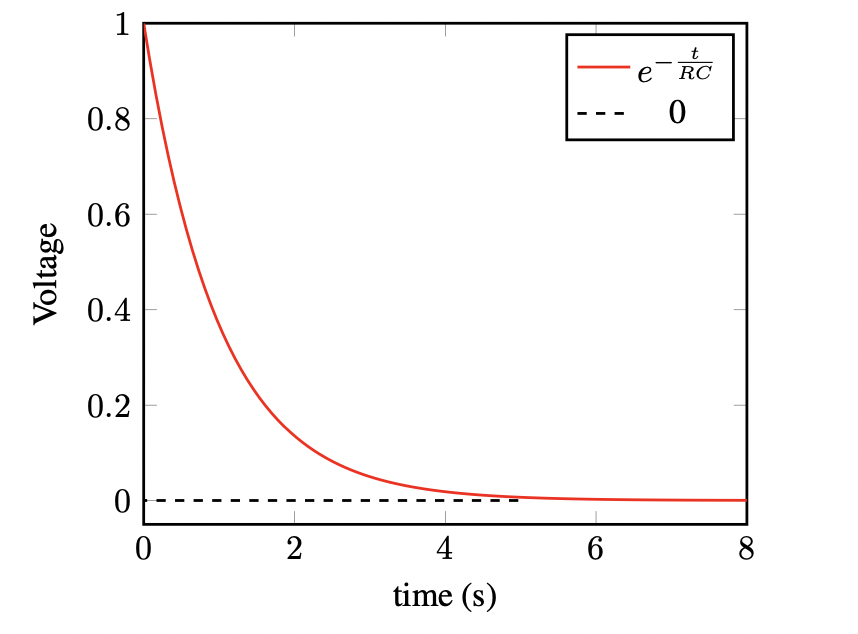
\includegraphics[scale=.6]{02-diffeq/discharge-graph.png}
    \caption{Voltage on discharging capacitor over time}
\end{figure}

\subsection{Uniqueness}

Our scalar and homogenous equations both had an arbitrary constant in their expression 
\begin{align*}
    x(t)&=bt+k_1\\
    x(t)&=k_2e^{at}
\end{align*}

Since any values of $k_1$ and $k_2$ satisfy their respective differential equations, that leaves us with a problem: there are an infinite number of possible solutions!

To restrict our set of solutions, we need more information. Specifically, we want to  know the initial condition, the value of $x$ at $t=0$. Suppose we know that $x(0)=c_0$. 

Then, for our scalar differential equation, we get \[x(0)=b\cdot 0+k_1=k_1=c_0\] so $k_1=c_0$.

For our homogenous differential equation, \[x(0)=k_2e^{a\cdot 0}=k_2\cdot 1=c_0\] so, similarly, $k_2=c_0$.

Looking back at our RC circuit, we know that, initially, the capacitors are charged to a voltage of $V_{DD}$, so $V(0)=V_{DD}$ and our solution would thus be \[V(t)=V_{DD}e^{-\frac t{RC}}\]

\subsection{Proof of uniqueness}

For our homogenous equation, we have found a solution that works. However, that was by an educated guess and not mathematical proof. Is that the only possible solution? Let's try to prove it.

Suppose that there is another solution $y(t)$ to the homogenous differential equation such that $\frac d{dt}y(t)=ay(t)$. We want to prove that $y(t)$ has to be exactly the same as $c_oe^{at}$. 

One way to do that is to show that the ratio $\frac{y(t)}{c_0e^{at}}=1$ everywhere. Since $c_0$ may cause problems because it can be zero, let's instead consider the ratio $\frac{y(t)}{e^{at}}$ and see if it is $c_0$ everywhere.

Let's take the derivative of this ratio:

\begin{align*}
    \frac d{dt}\frac {y(t)}{e^{at}}&=\frac d{dt}y(t)e^{-at}\\
    &=-ay(t)e^{-at}+e^{-at}\frac d{dt}y(t)\\
    &=-ay(t)e^{-at}+ay(t)e^{-at}\\
    &=0
\end{align*}

Since the derivative is always zero, the ratio must be a constant. But what constant? From the initial condition, we know that $y(0)=c_0$. Additionally, $e^{a\cdot 0}=1$, so the constant is $c_0/1$. In other words, we've proved that it is always true that \[\frac{y(t)}{e^{at}}=c_0\] so $y(t)=c_0e^{at}$ always too, and uniqueness is proved.

\subsection{Nonhomogenous differential equations}

Now let's take a look at nonhomogenous differential equations, in the form \[\frac d{dt}x(t)=ax+b\text{, where $b\ne 0$}\]

We solve this by doing a change of variables. Define \[\tilde x(t)=x(t)+\frac ba\]

Then, taking the derivative of that gets us 
\begin{align*}
    \frac d{dt}\tilde x(t)&=\frac d{dt}\left(x(t)+\frac ba\right)\\
    &=\frac d{dt}x(t)\\
    &=ax(t)+b\\
    &=a\left(\tilde x(t)-\frac ba\right)+b\\
    &=a\tilde x(t)
\end{align*}

This is just a homogenous equation now! Thus, know that $\tilde x(t)=ke^{at}$, so \[x(t)=ke^{at}-\frac ba\]

Plugging in our initial condition of $x(0)=c_0$ yields 
\begin{align*}
    c_0=x(0)&=ke^0-\frac ba\\
    k&=c_0+\frac ba
\end{align*}

Thus, our final equation is \[x(t)=(c_0+\frac ba)e^{at}-\frac ba\]

As an exercise, verify that this indeed satisfies the differential equation.

\subsubsection{Example: Charging RC circuit}

An example of this type of differential equation is when a capacitor charges up, or when an inverter switches from 0 to 1.

\begin{figure}[H]
    \centering
        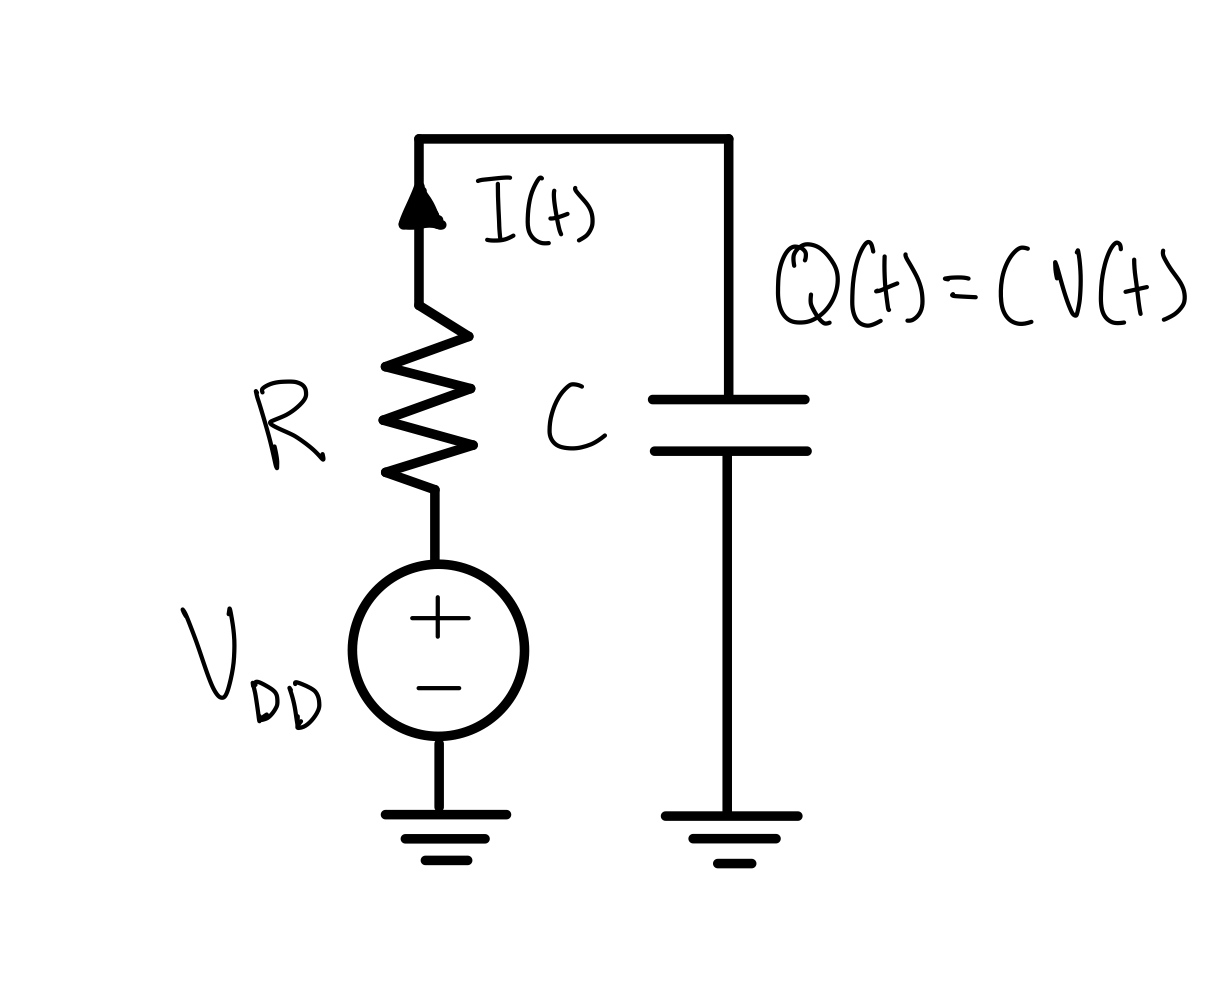
\includegraphics[scale=.15]{02-diffeq/charging-rc.jpeg}
    \caption{Capacitor charging through resistor}
\end{figure}

The differential equation that corresponds to the voltage of the capacitor here is \[\frac d{dt}V(t)=-\frac{V(t)}{RC}+\frac{V_{DD}}{RC}\]

I won't show the proof of that here but it is a good exercise to solve for it yourself by following the same steps as deriving the equation for a discharging capacitor.

In this case, $a=-\frac1{RC}$ and $b=\frac{V_{DD}}{RC}$. We substitute in $V(t)=\tilde V(t)+\frac{V_{DD}}{RC}\cdot\frac{-1}{RC}=\tilde V(t)+V_{DD}$ to get 

\begin{align*}
    \frac d{dt}\left(\tilde V(t)+V_{DD}\right)&=-\frac{\tilde V(t)+V_{DD}}{RC}+\frac{V_{DD}}{RC}\\
    \frac d{dt}\tilde V(t)&=-\frac{\tilde V(t)}{RC}\\
    \tilde V(t)&=ke^{-\frac t{RC}}\\
    V(t)&=ke^{-\frac t{RC}}+V_{DD}
\end{align*}

Using our initial condition $V(0)=0$, we get 
\begin{align*}
    0&=V(0)=ke^0+V_{DD}\\
    k&=-V_{DD}
\end{align*}

Thus our final solution to this differential equation is \[V(t)=V_{DD}(1-e^{-\frac t{RC}})\]

\begin{figure}[H]
    \centering
        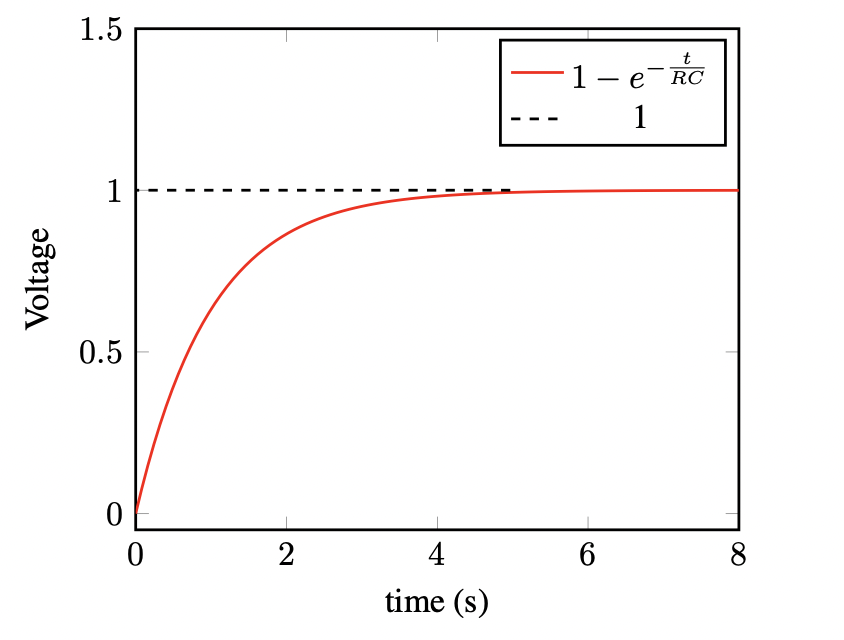
\includegraphics[scale=.6]{02-diffeq/charge-graph.png}
    \caption{Voltage on charging capacitor over time}
\end{figure}

\end{document}